\documentclass[landscape,final,a3paper,fontscale=1]{baposter}
\usepackage[utf8]{inputenc}
\usepackage{calc}
\usepackage{graphicx}
\usepackage{amsmath}
\usepackage{amssymb}
\usepackage{relsize}
\usepackage{multirow}
\usepackage{rotating}
\usepackage{bm}
\usepackage{url}

\usepackage{graphicx}
\usepackage{multicol}

% \setlength{\topmargin}{-7em}
%\usepackage{times}
%\usepackage{helvet}
%\usepackage{bookman}
\usepackage{palatino}

\newcommand{\captionfont}{\footnotesize}
\newcommand{\vect}[1]{\mathbf{#1}}

\graphicspath{{figures/}}
\usetikzlibrary{calc}

%%%%%%%%%%%%%%%%%%%%%%%%%%%%%%%%%%%%%%%%%%%%%%%%%%%%%%%%%%%%%%%%%%%%%%%%%%%%%%%%
%%%% Some math symbols used in the text
%%%%%%%%%%%%%%%%%%%%%%%%%%%%%%%%%%%%%%%%%%%%%%%%%%%%%%%%%%%%%%%%%%%%%%%%%%%%%%%%

%%%%%%%%%%%%%%%%%%%%%%%%%%%%%%%%%%%%%%%%%%%%%%%%%%%%%%%%%%%%%%%%%%%%%%%%%%%%%%%%
% Multicol Settings
%%%%%%%%%%%%%%%%%%%%%%%%%%%%%%%%%%%%%%%%%%%%%%%%%%%%%%%%%%%%%%%%%%%%%%%%%%%%%%%%
\setlength{\columnsep}{1.5em}
\setlength{\columnseprule}{0mm}

%%%%%%%%%%%%%%%%%%%%%%%%%%%%%%%%%%%%%%%%%%%%%%%%%%%%%%%%%%%%%%%%%%%%%%%%%%%%%%%%
% Save space in lists. Use this after the opening of the list
%%%%%%%%%%%%%%%%%%%%%%%%%%%%%%%%%%%%%%%%%%%%%%%%%%%%%%%%%%%%%%%%%%%%%%%%%%%%%%%%
\newcommand{\compresslist}{%
\setlength{\itemsep}{1pt}%
\setlength{\parskip}{0pt}%
\setlength{\parsep}{0pt}%
}

%%%%%%%%%%%%%%%%%%%%%%%%%%%%%%%%%%%%%%%%%%%%%%%%%%%%%%%%%%%%%%%%%%%%%%%%%%%%%%
%%% Begin of Document
%%%%%%%%%%%%%%%%%%%%%%%%%%%%%%%%%%%%%%%%%%%%%%%%%%%%%%%%%%%%%%%%%%%%%%%%%%%%%%

\begin{document}

%%%%%%%%%%%%%%%%%%%%%%%%%%%%%%%%%%%%%%%%%%%%%%%%%%%%%%%%%%%%%%%%%%%%%%%%%%%%%%
%%% Here starts the poster
%%%---------------------------------------------------------------------------
%%% Format it to your taste with the options
%%%%%%%%%%%%%%%%%%%%%%%%%%%%%%%%%%%%%%%%%%%%%%%%%%%%%%%%%%%%%%%%%%%%%%%%%%%%%%
% Define some colors

%\definecolor{lightblue}{cmyk}{0.83,0.24,0,0.12}
\definecolor{lightblue}{rgb}{0.145,0.6666,1}
\definecolor{lightgray}{rgb}{0.8509,0.8509,0.8510}
\definecolor{darkgray}{rgb}{0.7529,0.7529,0.7529}

%%
\begin{poster}%
  % Poster Options
  {
  % Show grid to help with alignment
  grid=false,
  % Column spacing
  colspacing=1em,
  % Color style
  bgColorOne=lightgray,
  bgColorTwo=white,
  borderColor=darkgray,
  headerColorOne=white,
  headerColorTwo=darkgray,
  headerFontColor=black,
  boxColorOne=white,
  boxColorTwo=darkgray,
  % Format of textbox
  textborder=roundedleft,
  % Format of text header
  eyecatcher=true,
  headerborder=closed,
  headerheight=0.11\textheight,
%  textfont=\sc, An example of changing the text font
  headershape=roundedright,
  headershade=shadelr,
  headerfont=\large\bf\textsc, %Sans Serif
  textfont={\setlength{\parindent}{1.5em}},
  boxshade=none,
%  background=shade-tb,
  background=shadelr,
  linewidth=1pt
  }
  % Eye Catcher
  {\includegraphics[height=8em]{wut_physics.png}} 
  % Title
  {\bf\textsc{\huge{Calculation of predictions for non-identical particle correlations in heavy ions\\\vspace{0.3em}collisions at LHC energies from hydrodynamics-inspired models}}\vspace{0.1em}}
  % Authors
  {\textsc{Mateusz Gałażyn\\\small{Faculty of Physics, Warsaw University of Technology}}}
  % University logo
  {% The makebox allows the title to flow into the logo, this is a hack because of the L shaped logo.
    \includegraphics[height=8em]{wut.png}
  }

%%%%%%%%%%%%%%%%%%%%%%%%%%%%%%%%%%%%%%%%%%%%%%%%%%%%%%%%%%%%%%%%%%%%%%%%%%%%%%
%%% Now define the boxes that make up the poster
%%%---------------------------------------------------------------------------
%%% Each box has a name and can be placed absolutely or relatively.
%%% The only inconvenience is that you can only specify a relative position 
%%% towards an already declared box. So if you have a box attached to the 
%%% bottom, one to the top and a third one which should be in between, you 
%%% have to specify the top and bottom boxes before you specify the middle 
%%% box.
%%%%%%%%%%%%%%%%%%%%%%%%%%%%%%%%%%%%%%%%%%%%%%%%%%%%%%%%%%%%%%%%%%%%%%%%%%%%%%
    %
    % A coloured circle useful as a bullet with an adjustably strong filling
    \newcommand{\colouredcircle}{%
      \tikz{\useasboundingbox (-0.2em,-0.32em) rectangle(0.2em,0.32em); \draw[draw=black,fill=lightblue,line width=0.03em] (0,0) circle(0.18em);}}

%%%%%%%%%%%%%%%%%%%%%%%%%%%%%%%%%%%%%%%%%%%%%%%%%%%%%%%%%%%%%%%%%%%%%%%%%%%%%%
  \headerbox{Abstract}{name=abstract,column=0,row=0}{
%%%%%%%%%%%%%%%%%%%%%%%%%%%%%%%%%%%%%%%%%%%%%%%%%%%%%%%%%%%%%%%%%%%%%%%%%%%%%%
    This thesis presents results of two-particle momentum correlations analysis for different kinds of particles produced in heavy ion collisions.
    The studies were carried for the data from lead-lead collisions at the centre of mass energy \mbox{$\sqrt{s_{NN}}=2.76$~TeV} simulated in the THERMINATOR model using the (3+1)-dimensional hydrodynamic model with viscosity.
    Analysis was performed for the three particle types: pions, kaons and protons for the collisions in eight different centrality ranges.
    Relativistic hydrodynamics predicts appearance of femtoscopic radii in the LCMS.
    This thesis concentrates on verification of such scaling and tests the possibility of scaling recovery in PRF.
    \vspace{1em}
  }
%%%%%%%%%%%%%%%%%%%%%%%%%%%%%%%%%%%%%%%%%%%%%%%%%%%%%%%%%%%%%%%%%%%%%%%%%%%%%%
  \headerbox{Heavy Ion Collisions}{name=hic,column=0,row=0,below=abstract}{
%%%%%%%%%%%%%%%%%%%%%%%%%%%%%%%%%%%%%%%%%%%%%%%%%%%%%%%%%%%%%%%%%%%%%%%%%%%%%%
    At the beginning, two thin discs are approaching to themselves nearly at the speed of light in order to collide with each other.
    In this reaction, energy stored in accelerated nuclei is used to investigate a strong interaction, a force which is binding nucleons into nuclei.
    Quantum Chromodynamics predicts an appearance of a new state of matter in relativistic heavy ion collisions - a quark-gluon plasma.
    Recent discoveries show, that this new state of matter behave like an ideal fluid and can be described by hydrodynamic equations.
    \\~\\
    \includegraphics[width=1\linewidth]{collision.png}
  }

%%%%%%%%%%%%%%%%%%%%%%%%%%%%%%%%%%%%%%%%%%%%%%%%%%%%%%%%%%%%%%%%%%%%%%%%%%%%%%
  \headerbox{Calculation Method}{name=method,column=0,span=2,row=0,below=hic,above=bottom}{
%%%%%%%%%%%%%%%%%%%%%%%%%%%%%%%%%%%%%%%%%%%%%%%%%%%%%%%%%%%%%%%%%%%%%%%%%%%%%%
    \begin{multicols}{2}
      Experimental correlation function is calculated from simulated data using following formula:
      \begin{equation}
        \label{experimental_cf}
        C(\vect{k^*}) = \frac{N}{D} =  \frac{\sum\limits_{n_i \in D} \delta(\vect{k^*}_i - \vect{k^*}) |\Psi_{ab}(\vect{r^*}_i,\vect{k^*}_i)|^2 }{\sum\limits_{n_i \in D} \delta(\vect{k^*}_i - \vect{k^*})}~,
      \end{equation}
      where \textit{N} and \textit{D} are three dimensional histograms of a particle pairs relative momentum $2k^*$ and $\Psi_{ab}$ is a pair wave function.
      In order to carry out multi-dimensional analysis of a correlation function, a decomposition into spherical harmonics series was performed:
      \begin{equation}
      \label{cf_dec}
      C(\vect{q}) = \sum_{l,m} C^m_l (q) Y^m_l(\theta, \phi),
      \end{equation}
      \begin{equation}
      C^m_l(q) = \int_\Omega C(q,\theta,\phi) Y^{m*}_l (\theta,\phi) d \Omega~,
      \end{equation}
      where $Y_{l}^{m}$ is spherical harmonic, $\textbf{q}$ is a pair momentum difference, $\Theta$ and $\phi$ are spherical coordinates.
    \end{multicols}
  }  

%%%%%%%%%%%%%%%%%%%%%%%%%%%%%%%%%%%%%%%%%%%%%%%%%%%%%%%%%%%%%%%%%%%%%%%%%%%%%%
  \headerbox{Particle Interferometry}{name=femtoscopy,column=1,row=0}{
%%%%%%%%%%%%%%%%%%%%%%%%%%%%%%%%%%%%%%%%%%%%%%%%%%%%%%%%%%%%%%%%%%%%%%%%%%%%%%
    Two-particle interferometry (also called femtoscopy) gives a possibility to investigate space-time characteristics of the emitting source.
    Through the study of two-particle correlations, their momentum distributions can be used to obtain information about the extent of created system.
    This method allows to measure sizes of the order of $10^{-15}$ m and time of the order of $10^{-23}$ s.
    \\~\\
    \includegraphics[width=1\linewidth]{pairs.png}
  }

%%%%%%%%%%%%%%%%%%%%%%%%%%%%%%%%%%%%%%%%%%%%%%%%%%%%%%%%%%%%%%%%%%%%%%%%%%%%%%
  \headerbox{THERMINATOR Model}{name=therminator,column=1,row=0,below=femtoscopy,above=method}{
%%%%%%%%%%%%%%%%%%%%%%%%%%%%%%%%%%%%%%%%%%%%%%%%%%%%%%%%%%%%%%%%%%%%%%%%%%%%%%
    THERMINATOR is a Monte Carlo event generator designed for studying of the statistical production of particles in relativistic heavy ion collisions.
    The creation of stable particles and unstable resonances (hadronisation) is determined by statistical (Bose-Einstein and Fermi-Dirac) distribution factors.
    After the hadronisation phase, the THERMINATOR provides space-time evolution and resonances decays in cascades.
    The key element of this approach is the inclusion of the complete list of hadronic short-time living resonances, which at the rather high temperature at freeze-out ($T_f \approx 165 MeV$) contribute very significantly to the observed particles.
    This code does not take into account interactions between final state hadrons.
    THERMINATOR is written in C++ language and uses the CERN ROOT environment.
  }    

%%%%%%%%%%%%%%%%%%%%%%%%%%%%%%%%%%%%%%%%%%%%%%%%%%%%%%%%%%%%%%%%%%%%%%%%%%%%%%
\headerbox{Experimental Correlation Functions}{name=res-id,column=2,span=2,row=0}{
%%%%%%%%%%%%%%%%%%%%%%%%%%%%%%%%%%%%%%%%%%%%%%%%%%%%%%%%%%%%%%%%%%%%%%%%%%%%%%
  \begin{multicols}{2}
    The correlation functions (three- and one-dimensional) were calculated separately for the following different pairs of identical particles: $\pi$-$\pi$, $K$-$K$ and  $p$-$p$ for nine $k_T$ bins (in ) from 0.1~GeV/c to 1.2~GeV/c.
    The three-dimensional correlation function as a function of relative momentum $q_{LCMS}$ was calculated in a form of components of spherical harmonics series accordingly to Eq.~\ref{cf_dec}.
    In the femtoscopic analysis of identical particles, the most important information is stored in the $\Re C^0_0$, $\Re C^0_2$ and $\Re C^2_2$, hence only these components were analyzed.
    Correlation functions obtained in this procedure were calculated for the pairs of pions, kaons and protons in the different centrality bins.
    Particular coefficients for pairs of identical bosons (pions and kaons) are shown in the plot on the right side.
    The wave function symmetrization (Bose-Einstein statistics) causes the increase of correlation in the low relative momenta regime.
    The $\Re C_0^0$ resembles one-dimensional correlation function in the sense that it encodes information about the overall source radius.
    The second coefficient $\Re C^0_2$ differs from zero (is negative), which yields the information about the ratio $R_T / R_{long}$.
    The $\Re C^2_2$ stores the information about $R_{out} / R_{side}$ ratio and one can notice that is non-vanishing (is also negative).
    ~\\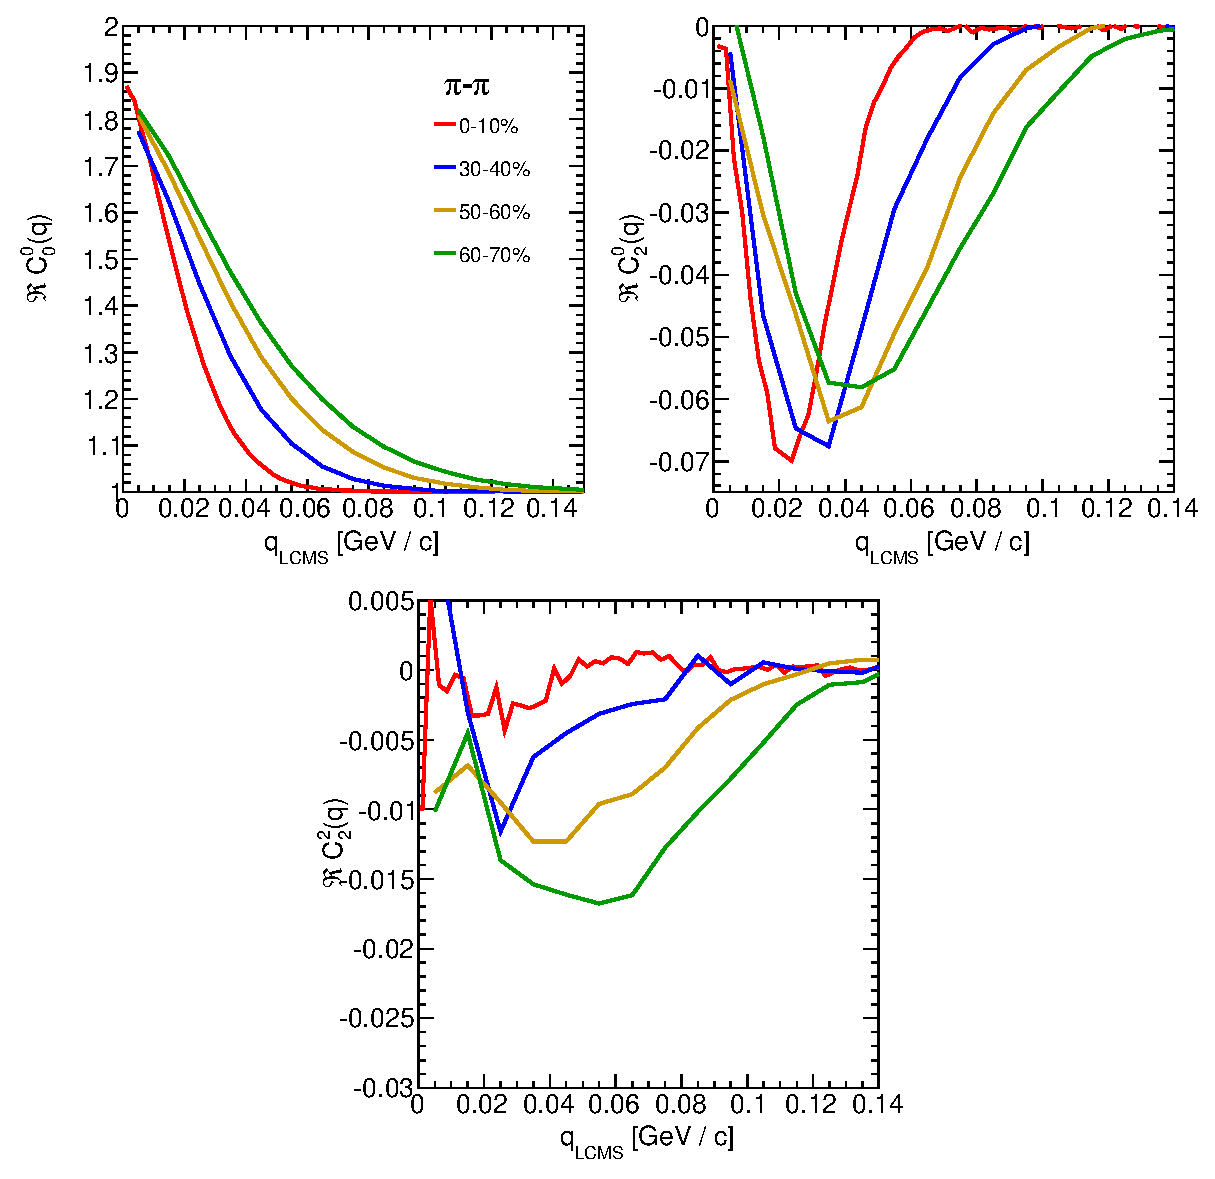
\includegraphics[width=1\linewidth]{results/cf3dpi}
  \end{multicols}
}
%%%%%%%%%%%%%%%%%%%%%%%%%%%%%%%%%%%%%%%%%%%%%%%%%%%%%%%%%%%%%%%%%%%%%%%%%%%%%%
\headerbox{Results for Radii Scaling}{name=res-radii,column=2,span=2,row=0,below=res-id,above}{
%%%%%%%%%%%%%%%%%%%%%%%%%%%%%%%%%%%%%%%%%%%%%%%%%%%%%%%%%%%%%%%%%%%%%%%%%%%%%%
    \begin{multicols}{2}
      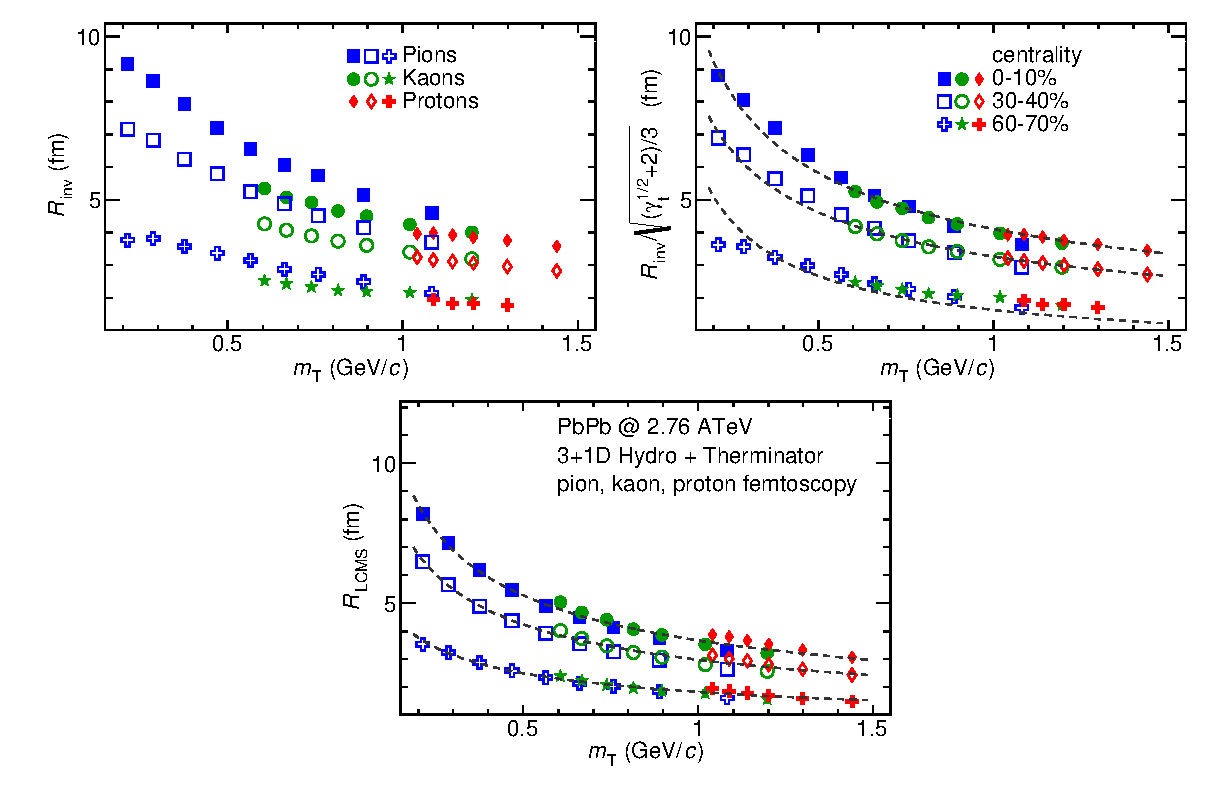
\includegraphics[width=1\linewidth]{results/scaling_test}
      From identical particles correlation functions one can extract femtoscopic radii ($R$) - ranges of correlation effect between particles.
      Calculations of a correlation function can be performed in two coordinate systems: Pair Rest Frame and Longitudinally Co-moving System.
      Hydrodynamics predict the following rule: $R_{LCMS} = \alpha m_T^{-\gamma}$, where $m_T$ is a transverse mass, $\alpha$ and $\gamma$ are parameters.
      Plots on the right side present femtoscopic radii from PRF (upper left) and LCMS (lower one). Upper right plot present results in PRF divided by proposed scaling factor: $\left[ \left( \sqrt{\gamma_t} + 2 \right) / 3 \right]^{-1/2}$, lower plots are in LCMS.
      One can notice that the femtoscopic radii are falling on the common curve after division.
    \end{multicols}
}
%%%%%%%%%%%%%%%%%%%%%%%%%%%%%%%%%%%%%%%%%%%%%%%%%%%%%%%%%%%%%%%%%%%%%%%%%%%%%%
  \headerbox{Conclusions}{name=conclusions,column=2,span=2,below=res-radii,above=bottom}{
%%%%%%%%%%%%%%%%%%%%%%%%%%%%%%%%%%%%%%%%%%%%%%%%%%%%%%%%%%%%%%%%%%%%%%%%%%%%%%
  \begin{multicols}{2}
  Hydrodynamic equations are predicting appearance of the common scaling of femtoscopic radii for different kinds of particles with $m_T^{-0.5}$ in LCMS.
  In the results of this work, a common scaling for different particle types is observed in LCMS in the outward, sideward and longitudinal directions.
  The direction-averaged radius $R_{LCMS}$ also shows this power-law behaviour.
  The fitting of a power-law $\alpha m_T^{-\beta}$ to the femtoscopic radii yielded the information that the $\beta$ exponent for the outward and sideward directions is of the order of 0.5, which is consistent with the hydrodynamic predictions.
  For the longitudinal direction, the $\beta$ is bigger (>0.7) than in the other ones, which is an indication of a strong transverse flow.
  
  In the case of the one-dimensional radii $R_{inv}$ calculated in PRF, no common scaling is observed.
  However, one can try to correct the influence of the $R_{out}$ growth with an approximate factor $\sqrt{ \left. \left( \sqrt{\gamma_T} + 2 \right) \middle/ 3 \right. }$.
  After the division of the $R_{inv}$ by the proposed factor, the scaling is restored with an accuracy <~10\%.
  In this way, the experimentally simpler measure of the one-dimensional radii can be used as a probe for the hydrodynamic collectivity.
  \end{multicols}
  }

\end{poster}

\end{document}
